\documentclass[landscape,final,paperwidth=48in,paperheight=36in]{baposter}

\usepackage{calc}
\usepackage{graphicx}
\usepackage{amsmath}
\usepackage{amssymb}
\usepackage{relsize}
\usepackage{multirow}
\usepackage{rotating}
\usepackage{bm}
\usepackage{url} 

\usepackage{amsthm} 
\usepackage{amssymb}
\usepackage{amsmath}

\newtheorem{conjecture}{Conjecture}
\newtheorem{example}{Example}
\newtheorem{definition}{Definition}
\newtheorem{proposition}{Proposition}
\newtheorem{lemma}{Lemma}
\newtheorem{theorem}{Theorem}

\usepackage{graphicx}
\usepackage{multicol}

%\usepackage{times}
%\usepackage{helvet}
%\usepackage{bookman}
\usepackage{palatino}

\newcommand{\captionfont}{\footnotesize}

\graphicspath{{images/}{../images/}}
\usetikzlibrary{calc}

\newcommand{\SET}[1]  {\ensuremath{\mathcal{#1}}}
\newcommand{\MAT}[1]  {\ensuremath{\boldsymbol{#1}}}
\newcommand{\VEC}[1]  {\ensuremath{\boldsymbol{#1}}}
\newcommand{\Video}{\SET{V}}
\newcommand{\video}{\VEC{f}}
\newcommand{\track}{x}
\newcommand{\Track}{\SET T}
\newcommand{\LMs}{\SET L}
\newcommand{\lm}{l}
\newcommand{\PosE}{\SET P}
\newcommand{\posE}{\VEC p}
\newcommand{\negE}{\VEC n}
\newcommand{\NegE}{\SET N}
\newcommand{\Occluded}{\SET O}
\newcommand{\occluded}{o}

%%%%%%%%%%%%%%%%%%%%%%%%%%%%%%%%%%%%%%%%%%%%%%%%%%%%%%%%%%%%%%%%%%%%%%%%%%%%%%%%
%%%% Some math symbols used in the text
%%%%%%%%%%%%%%%%%%%%%%%%%%%%%%%%%%%%%%%%%%%%%%%%%%%%%%%%%%%%%%%%%%%%%%%%%%%%%%%%

%%%%%%%%%%%%%%%%%%%%%%%%%%%%%%%%%%%%%%%%%%%%%%%%%%%%%%%%%%%%%%%%%%%%%%%%%%%%%%%%
% Multicol Settings
%%%%%%%%%%%%%%%%%%%%%%%%%%%%%%%%%%%%%%%%%%%%%%%%%%%%%%%%%%%%%%%%%%%%%%%%%%%%%%%%
\setlength{\columnsep}{1.5em}
\setlength{\columnseprule}{0mm}

%%%%%%%%%%%%%%%%%%%%%%%%%%%%%%%%%%%%%%%%%%%%%%%%%%%%%%%%%%%%%%%%%%%%%%%%%%%%%%%%
% Save space in lists. Use this after the opening of the list
%%%%%%%%%%%%%%%%%%%%%%%%%%%%%%%%%%%%%%%%%%%%%%%%%%%%%%%%%%%%%%%%%%%%%%%%%%%%%%%%
\newcommand{\compresslist}{%
\setlength{\itemsep}{1pt}%
\setlength{\parskip}{0pt}%
\setlength{\parsep}{0pt}%
}

%%%%%%%%%%%%%%%%%%%%%%%%%%%%%%%%%%%%%%%%%%%%%%%%%%%%%%%%%%%%%%%%%%%%%%%%%%%%%%
%%% Begin of Document
%%%%%%%%%%%%%%%%%%%%%%%%%%%%%%%%%%%%%%%%%%%%%%%%%%%%%%%%%%%%%%%%%%%%%%%%%%%%%%

\begin{document}

%%%%%%%%%%%%%%%%%%%%%%%%%%%%%%%%%%%%%%%%%%%%%%%%%%%%%%%%%%%%%%%%%%%%%%%%%%%%%%
%%% Here starts the poster
%%%---------------------------------------------------------------------------
%%% Format it to your taste with the options
%%%%%%%%%%%%%%%%%%%%%%%%%%%%%%%%%%%%%%%%%%%%%%%%%%%%%%%%%%%%%%%%%%%%%%%%%%%%%%
% Define some colors

%\definecolor{lightblue}{cmyk}{0.83,0.24,0,0.12}
\definecolor{lightblue}{rgb}{0.145,0.6666,1}

% Draw a video
\newlength{\FSZ}
\newcommand{\drawvideo}[3]{% [0 0.25 0.5 0.75 1 1.25 1.5]
   \noindent\pgfmathsetlength{\FSZ}{\linewidth/#2}
   \begin{tikzpicture}[outer sep=0pt,inner sep=0pt,x=\FSZ,y=\FSZ]
   \draw[color=lightblue!50!black] (0,0) node[outer sep=0pt,inner sep=0pt,text width=\linewidth,minimum height=0] (video) {\noindent#3};
   \path [fill=lightblue!50!black,line width=0pt] 
     (video.north west) rectangle ([yshift=\FSZ] video.north east) 
    \foreach \x in {1,2,...,#2} {
      {[rounded corners=0.6] ($(video.north west)+(-0.7,0.8)+(\x,0)$) rectangle +(0.4,-0.6)}
    }
;
   \path [fill=lightblue!50!black,line width=0pt] 
     ([yshift=-1\FSZ] video.south west) rectangle (video.south east) 
    \foreach \x in {1,2,...,#2} {
      {[rounded corners=0.6] ($(video.south west)+(-0.7,-0.2)+(\x,0)$) rectangle +(0.4,-0.6)}
    }
;
   \foreach \x in {1,...,#1} {
     \draw[color=lightblue!50!black] ([xshift=\x\linewidth/#1] video.north west) -- ([xshift=\x\linewidth/#1] video.south west);
   }
   \foreach \x in {0,#1} {
     \draw[color=lightblue!50!black] ([xshift=\x\linewidth/#1,yshift=1\FSZ] video.north west) -- ([xshift=\x\linewidth/#1,yshift=-1\FSZ] video.south west);
   }
   \end{tikzpicture}
}

\hyphenation{resolution occlusions}
%%
\begin{poster}%
  % Poster Options
  {
  % Show grid to help with alignment
  grid=false,
  % Column spacing
  colspacing=1em,
  % Color style
  bgColorOne=white,
  bgColorTwo=white,
  borderColor=lightblue,
  headerColorOne=black,
  headerColorTwo=lightblue,
  headerFontColor=white,
  boxColorOne=white,
  boxColorTwo=lightblue,
  % Format of textbox
  textborder=roundedleft,
  % Format of text header
  eyecatcher=true,
  headerborder=closed,
  headerheight=0.1\textheight,
%  textfont=\sc, An example of changing the text font
  headershape=roundedright,
  headershade=shadelr,
  headerfont=\Large\bf\textsc, %Sans Serif
  textfont={\setlength{\parindent}{1.5em}},
  boxshade=plain,
%  background=shade-tb,
  background=plain,
  linewidth=2pt
  }
  % Eye Catcher
  {
\includegraphics[height=8em,keepaspectratio=true]{images/logo_uprrp}} 
  % Title
  {\bf\textsc{On a Class of Permutation Polynomials}\vspace{0.1em}}
  % Authors
  {\textsc{Christian A. Rodr\'{\i}guez \& Alex D. Santos \\ University of Puerto Rico, Rio Piedras \\ Department of Computer Science}}
  % University logo
  {% The makebox allows the title to flow into the logo, this is a hack because of the L shaped logo.
    
\includegraphics[height=9em,keepaspectratio=true]{images/logo_ccom}
  }

%%%%%%%%%%%%%%%%%%%%%%%%%%%%%%%%%%%%%%%%%%%%%%%%%%%%%%%%%%%%%%%%%%%%%%%%%%%%%%
%%% Now define the boxes that make up the poster
%%%---------------------------------------------------------------------------
%%% Each box has a name and can be placed absolutely or relatively.
%%% The only inconvenience is that you can only specify a relative position 
%%% towards an already declared box. So if you have a box attached to the 
%%% bottom, one to the top and a third one which should be in between, you 
%%% have to specify the top and bottom boxes before you specify the middle 
%%% box.
%%%%%%%%%%%%%%%%%%%%%%%%%%%%%%%%%%%%%%%%%%%%%%%%%%%%%%%%%%%%%%%%%%%%%%%%%%%%%%
    %
    % A coloured circle useful as a bullet with an adjustably strong filling
    \newcommand{\colouredcircle}{%
      \tikz{\useasboundingbox (-0.2em,-0.32em) rectangle(0.2em,0.32em); \draw[draw=black,fill=lightblue,line width=0.03em] (0,0) circle(0.18em);}}

%%%%%%%%%%%%%%%%%%%%%%%%%%%%%%%%%%%%%%%%%%%%%%%%%%%%%%%%%%%%%%%%%%%%%%%%%%%%%%
  \headerbox{Abstract}{name=abstract,column=0,row=0}{
%%%%%%%%%%%%%%%%%%%%%%%%%%%%%%%%%%%%%%%%%%%%%%%%%%%%%%%%%%%%%%%%%%%%%%%%%%%%%%
   A polynomial $f(x)$ defined over a set $A$ is called a \textbf{permutation polynomial} if $f(x)$ acts as a permutation over the elements of $A$. This is, if $f: A \rightarrow A$ is 1-1 and onto. We are studying the coefficients $a$ and $b$ that make polynomials of the form $F_{a,b}(x)=x^{\frac{p+1}{2}} + ax^{\frac{p+5}{6}} + bx$ a permutation polynomial where $a,b \in \mathbb{F}_{q}^{\times}$. More specifically we study the family of polynomials: $F_{a,b}(x)=x^{\frac{p+1}{2}} + ax^{\frac{p+5}{6}} + bx$. Our approach in studying $F(x)$ is to use the division algorithm to consider $x=\alpha^{n}$ where $n=6k+r, r=0,...,5$. If $F_{a,b}(x)$ is a permutation, this partitions $\mathbb{F}_{q}^{\times}$ into 6 classes: $F_{a,b}(\alpha^{6k+r})$ for $r=0,...,5$.
   \vspace{0.3em}
 }\label{Abstract}

%%%%%%%%%%%%%%%%%%%%%%%%%%%%%%%%%%%%%%%%%%%%%%%%%%%%%%%%%%%%%%%%%%%%%%%%%%%%%%
  \headerbox{Value set of a class of polynomials}{name=contribution,column=1,row=0,span=2}{
%%%%%%%%%%%%%%%%%%%%%%%%%%%%%%%%%%%%%%%%%%%%%%%%%%%%%%%%%%%%%%%%%%%%%%%%%%%%%%
  \begin{multicols}{2}
    Our interest is studying the value set of a specific class of permutation polynomials. The class of polynomials we consider is defined as follows:
    $$F_{a,b}(x) = x^{\frac{q+1}{2}} + a\cdot x^{\frac{q+1}{d}} + b\cdot x$$
    
    Where $a,b \in \mathbb{F}_{q}$ and $d \mid q-1$. More formally, we would like to characterize the value set $V_{F}$ of $F_{a,b}(x)$ based on the parameters $a$ and $b$. It is easy to see that $F_{a,b}(0) = 0 \ \forall a,b \in \mathbb{F}_{q}$, it follows that $0$ is always in $V_{F}$. For a fixed pair $a,b$ we separate $V_{F} \setminus \left\{0\right\}$ into smaller subsets in the following way:

    \begin{definition}
      Let $F_{a,b}(x) = x^{\frac{q+1}{2}} + a\cdot x^{\frac{q+1}{d}} + b\cdot x$ be a polynomial defined over $\mathbb{F}_{q}$ where $d \mid q-1$. We define the sets $A_i = \left\{F_{a,b}(\alpha^{d\cdot k+i}) \mid k=0,...,\frac{q-1}{d}\right\}$ for $i=0,...,d-1$, where $\alpha$ is a primitive root of $\mathbb{F}_{q}$.
    \end{definition}

    Using properties of these sets we will characterize $V_{F}$. First we would like to note that for $i \neq j$ the sets $A_i$ and $A_j$ are either equal, or distinct.

    \begin{lemma}\label{conjuntos_disjuntos}
      Let $F_{a,b}(x)$ be defined over $\mathbb{F}_{q}$. For two sets $A_i$ and $A_j$ we must have that either $A_i \cap A_j = \emptyset$ or $A_i = A_j$.
    \end{lemma}

    Lemma~\ref{conjuntos_disjuntos} provides an immediate characterization of the value set and insight on conditions to make $F_{a,b}(x)$ a permutation polynomial. In our studies we also determine the size of the sets $A_i$.

    \begin{lemma}\label{tamanos_conjuntos}
      Let $F_{a,b}(x)$ be defined over $\mathbb{F}_{q}$ and $A_i$ be defined as above. We have that $\left\vert A_i \right\vert = \frac{q-1}{d}$ or $A_i = \left\{ 0 \right\}$
    \end{lemma}

    Now we are also interested in correlations between the pairs $a,b$ and the value sets of distinct polynomials of the for $F_{a,b}(x)$. We proved a lemma that gives us a correspondence among some of these polynomials. In other words, these polynomials have the same value set.

    \begin{lemma}\label{correspondencia}
      Let $F_{a,b}(x)$ defined over $\mathbb{F}_{q}$ and let $\alpha$ denote a primitive root of $\mathbb{F}_{q}$. If we write $a = \alpha^i$ and $b = \alpha^j$ then we have that
      $$F_{\alpha^i,\alpha^j}(\alpha^k) = -\alpha \cdot F_{\alpha^{i+(d+2)\cdot \frac{q-1}{2d}}, \alpha^{j+\frac{q-1}{2}}}(\alpha^{k-1})$$
    \end{lemma}

    From lemma~\ref{conjuntos_disjuntos} we know that for a fixed polynomial the sets $A_i$ are either distinct or equal. Finally from lemma~\ref{correspondencia} we have that up to $2d$ distinct polynomials of the form $F_{a,b}(x)$ have the same value set. This information gives us the following theorem:

    \begin{proposition}\label{el_teorema}
      Let $F_{a,b}(x)$ be defined over $\mathbb{F}_{q}$. Then we have that the amount of polynomials of the form $F_{a,b}(x)$ such that $\left\vert V_{F} \right\vert = r\cdot \frac{q-1}{d} + 1, r \leq d$ is divisible by $d$ when $d$ is even and by $2d$ when $d$is odd.
    \end{proposition}

  \end{multicols}

   \vspace{0.3em}
  }\label{Value sets}

%%%%%%%%%%%%%%%%%%%%%%%%%%%%%%%%%%%%%%%%%%%%%%%%%%%%%%%%%%%%%%%%%%%%%%%%%%%%%%
\headerbox{Applications}{name=applications,column=3,row=0}{
  %%%%%%%%%%%%%%%%%%%%%%%%%%%%%%%%%%%%%%%%%%%%%%%%%%%%%%%%%%%%%%%%%%%%%%%%%%%%%%
    \drawvideo{5}{40}{%
      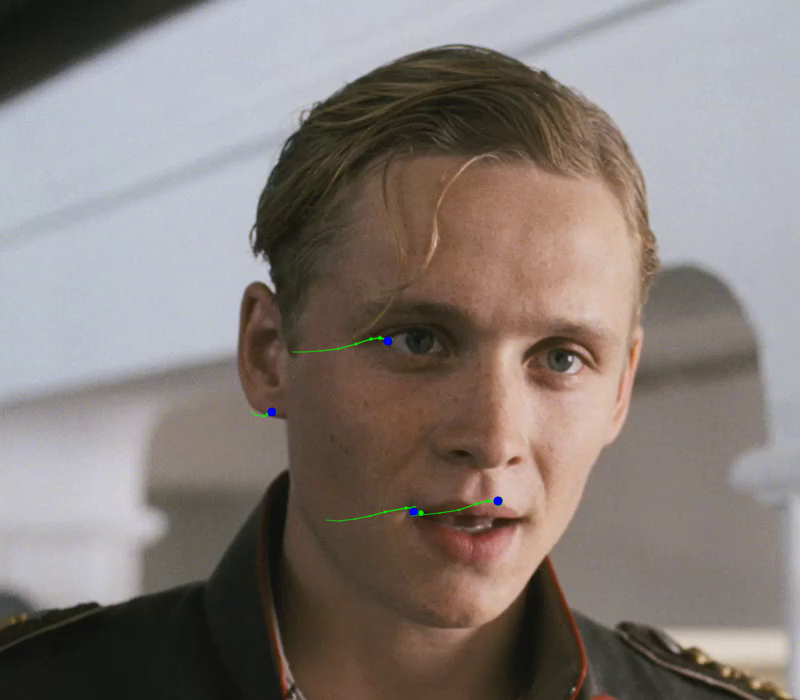
\includegraphics[width=0.2\linewidth]{red-4-sec_000_rastered}%
        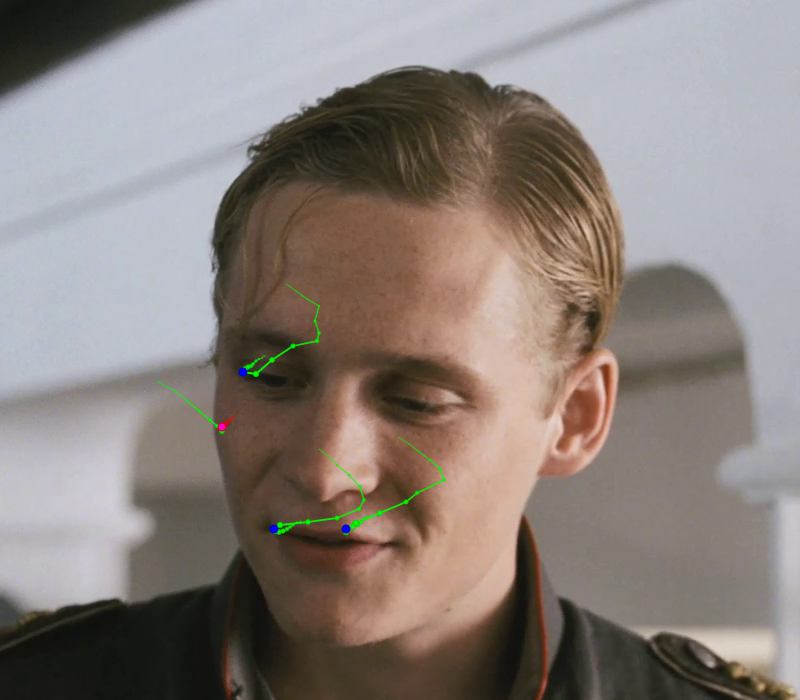
\includegraphics[width=0.2\linewidth]{red-4-sec_024_rastered}%
        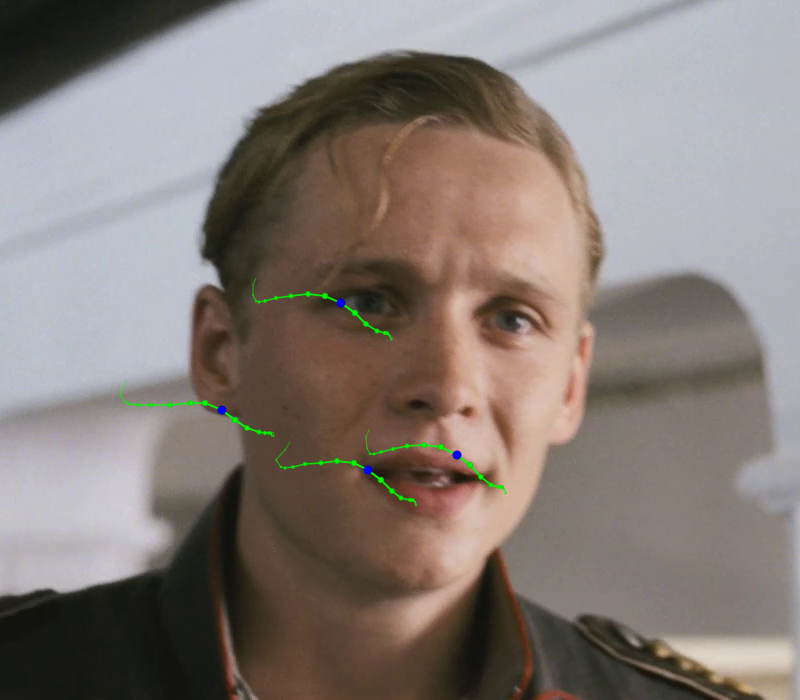
\includegraphics[width=0.2\linewidth]{red-4-sec_048_rastered}%
        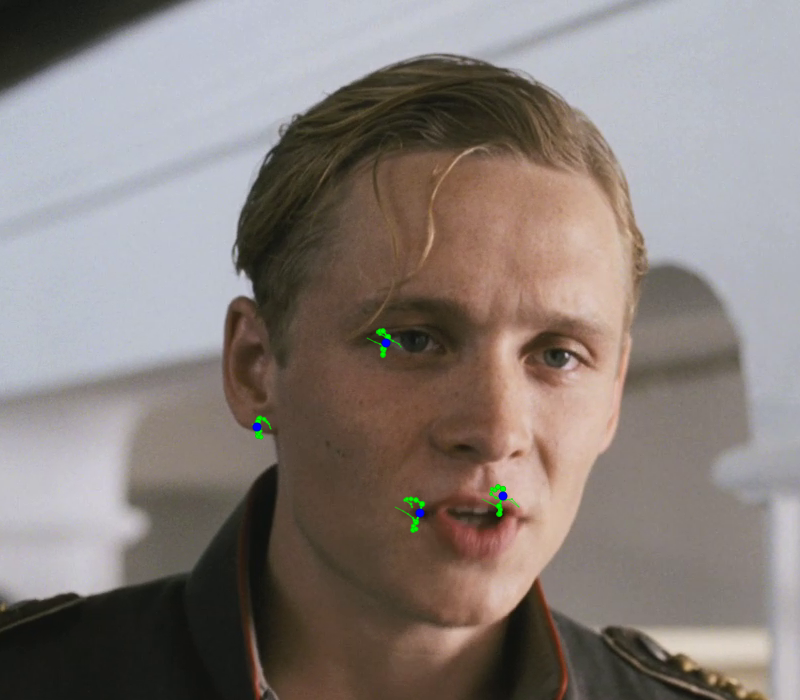
\includegraphics[width=0.2\linewidth]{red-4-sec_072_rastered}%
        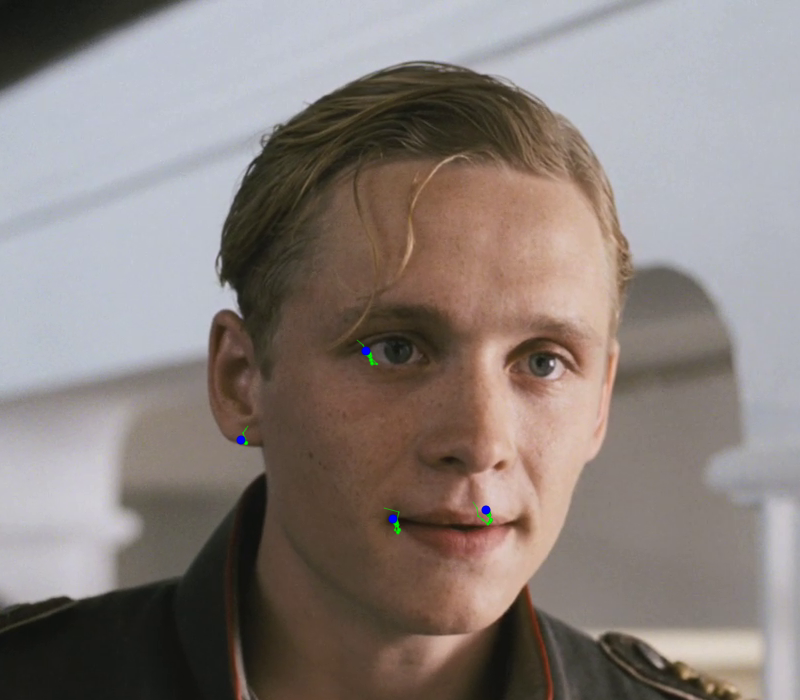
\includegraphics[width=0.2\linewidth]{red-4-sec_095_rastered}%
    }
  \begin{tabular*}{\linewidth}{*{5}{@{}p{0.2\linewidth}@{}}}
    {\hfill{}Frame 0\hfill{}} & {\hfill{}24\hfill{}} &  {\hfill{}48\hfill{}} &  {\hfill{}72\hfill{}} & {\hfill{}95\hfill{}}
  \end{tabular*}
  \\[1em]
      \drawvideo{5}{40}{%
        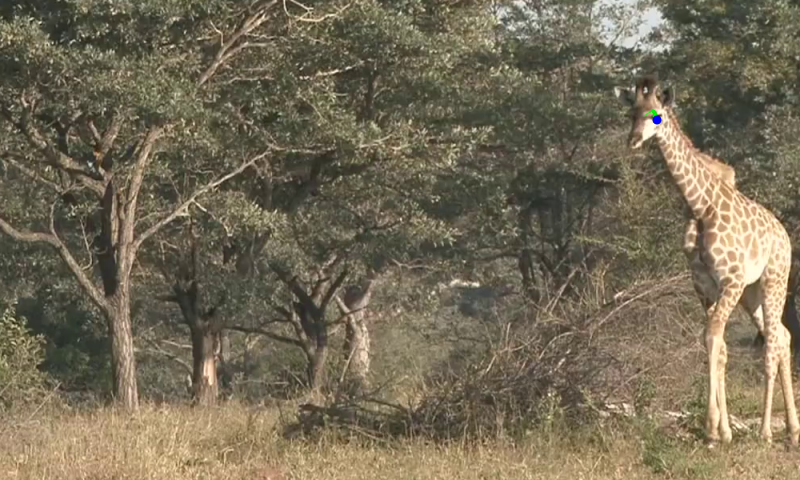
\includegraphics[width=0.2\linewidth]{giraffe-run-000-rastered}%
          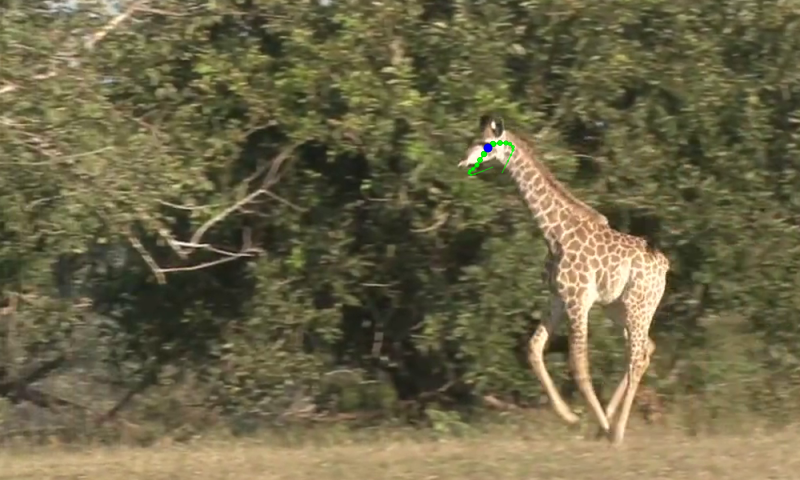
\includegraphics[width=0.2\linewidth]{giraffe-run-100-rastered}%
          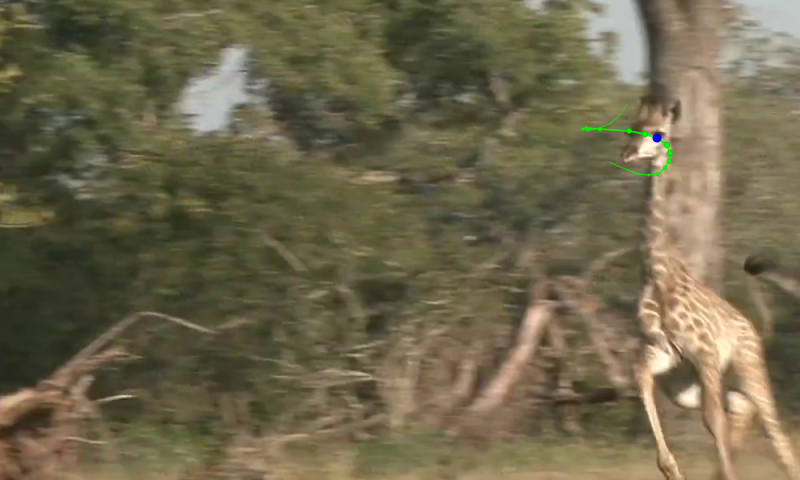
\includegraphics[width=0.2\linewidth]{giraffe-run-200-rastered}%
          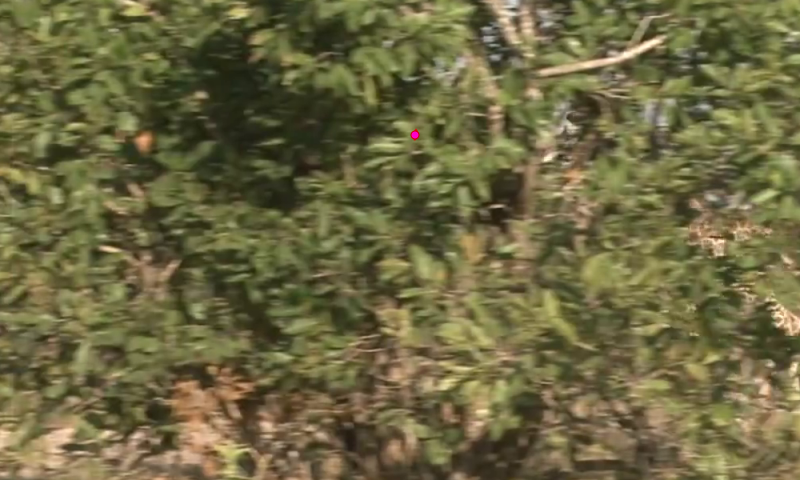
\includegraphics[width=0.2\linewidth]{giraffe-run-300-rastered}%
          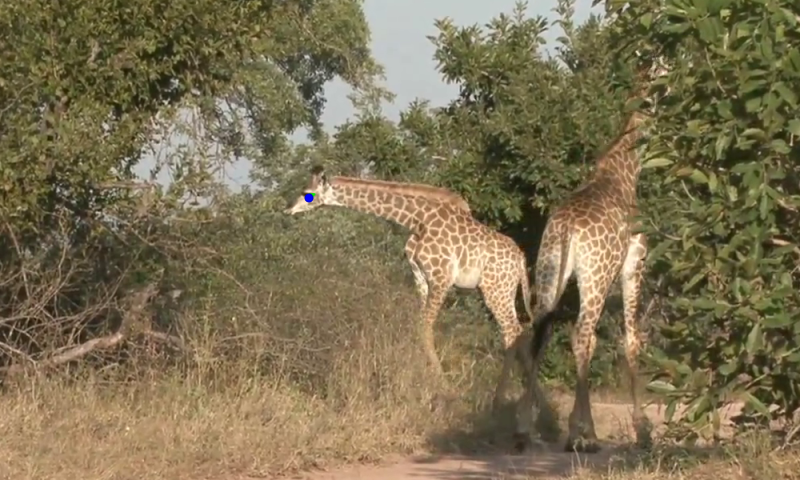
\includegraphics[width=0.2\linewidth]{giraffe-run-458-rastered}%
      }
  \begin{tabular*}{\linewidth}{*{5}{@{}p{0.2\linewidth}@{}}}
    {\hfill{}Frame 0\hfill{}}  &
    {\hfill{}100\hfill{}} &
    {\hfill{}200\hfill{}} &
    {\hfill{}300\hfill{}} &
    {\hfill{}458\hfill{}} 
  \end{tabular*}
      \begin{multicols}{2}
    Between one and three user clicks were needed to achieve accurate tracking for
      the head sequence. Note the correct handling of the occluded ear, which
      required only a single click. 

      The eye of the running giraffe required eight user interactions, of which three
      marked occlusions. 
      \end{multicols}
      \vspace{-0.6em}
}\label{Applications}

%%%%%%%%%%%%%%%%%%%%%%%%%%%%%%%%%%%%%%%%%%%%%%%%%%%%%%%%%%%%%%%%%%%%%%%%%%%%%%
  \headerbox{Preliminaries}{name=preliminaries,column=0,below=abstract,above=bottom}{
%%%%%%%%%%%%%%%%%%%%%%%%%%%%%%%%%%%%%%%%%%%%%%%%%%%%%%%%%%%%%%%%%%%%%%%%%%%%%%

We are interested in studying sets known as Finite Fields.

\begin{definition}
  A \textbf{Finite Field} $\mathbb{F}_{q}$ is a field with $q=p^r$ elements, where $p$ is a prime number.
\end{definition}

An important property of finite fields is the existence of a primitive root, a generator of the nonzero elements of $\mathbb{F}_q$.

\begin{definition}
  A \textbf{primitive root} $\alpha \in \mathbb{F}_q$ is a generator for the multiplicative group $\mathbb{F}_{q}^{\times}$
\end{definition}

\begin{example}
  Consider the finite field $\mathbb{F}_{7}$. We have that: $3^1 = 3, 3^2 = 2, 3^3 = 6, 3^4 = 4, 3^5 = 5, 3^6 = 1$, so $3$ is a primitive root of $\mathbb{F}_{7}$.
\end{example}

We are interested in studying polynomials defined over finite fields. Specifically, our interest lies in the value set of these polynomials.

\begin{definition}
  Let $f(x)$ be a polynomial defined over a finite field $\mathbb{F}_{q}$. Then the \textbf{value set} of $f$ is defined as $V_{f} = \left\{f(a) \mid a \in \mathbb{F}_{q} \right\}$
\end{definition}

In our work we characterize $V_{f}$ for a specific class of polynomials defined over finite fields. From this characterization we can provide information on the amount of permutation polynomials of our class.

\begin{definition}
  Consider a finite field $\mathbb{F}_{q}$. A polynomial $f(x)$ defined over $\mathbb{F}_{q}$ is said to be a permutation polynomial if $V_{f} = \mathbb{F}_{q}$.
\end{definition}

\begin{example}
  Consider the polynomial $f(x) = x+3$ defined over $\mathbb{F}_{7}$. We have that $f(0) = 3, f(1) = 4, f(2) = 5, f(3) = 6, f(4) = 0, f(5) = 1, f(6) = 2$, so $f(x)$ is a permutation polynomial over $\mathbb{F}_{7}$
\end{example}

   \vspace{0.3em}
}\label{Preliminaries}

%%%%%%%%%%%%%%%%%%%%%%%%%%%%%%%%%%%%%%%%%%%%%%%%%%%%%%%%%%%%%%%%%%%%%%%%%%%%%%
  \headerbox{Conditions for permutations of the from $F_{a,b}(x)$}{name=questions,column=1,span=2,above=bottom,below=contribution}{
%%%%%%%%%%%%%%%%%%%%%%%%%%%%%%%%%%%%%%%%%%%%%%%%%%%%%%%%%%%%%%%%%%%%%%%%%%%%%%
  \begin{multicols}{2}
    We incorporated a background model, where a click informs us not only that `this is how the
    patch looks like', but also for the rest of the frame, `this is how the patch
    does not look like'. 
    
    Can we also \emph{efficiently} use a background tracks model, allowing us
    to reason, `this would be a good track, but part of it can be better
    explained by tracking another point'.
  \end{multicols}
   \vspace{0.3em}
  }\label{Conditions for PP}

%%%%%%%%%%%%%%%%%%%%%%%%%%%%%%%%%%%%%%%%%%%%%%%%%%%%%%%%%%%%%%%%%%%%%%%%%%%%%%
  \headerbox{Future Work}{name=future work,column=3,below=applications}{
%%%%%%%%%%%%%%%%%%%%%%%%%%%%%%%%%%%%%%%%%%%%%%%%%%%%%%%%%%%%%%%%%%%%%%%%%%%%%%
\noindent\begin{tabular}{r@{\hspace{0.3em}}c@{\hspace{1.5em}}c@{}}
& With & Without\\
& background model & background model\\
\begin{sideways}{\makebox[0.37\linewidth][c]{Ridge of the lips}}\end{sideways} &
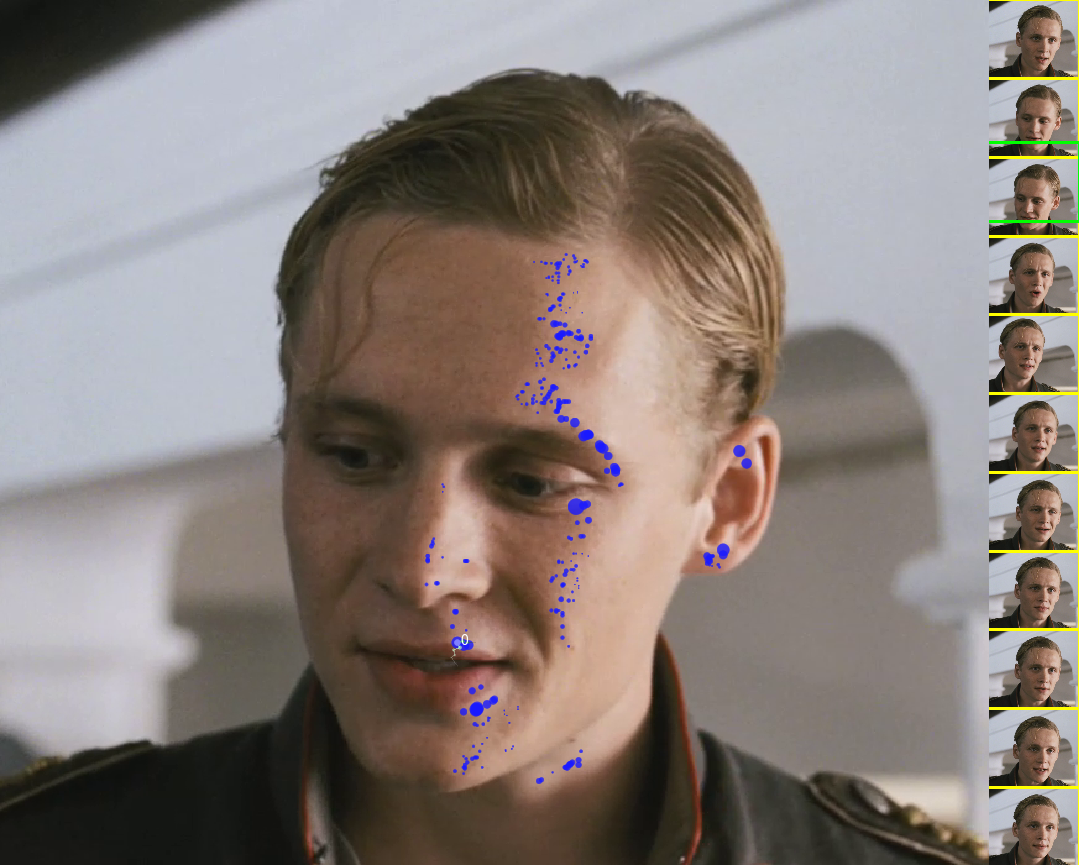
\includegraphics[width=0.40\linewidth]{candidates_lips_ridge_left_bg} &
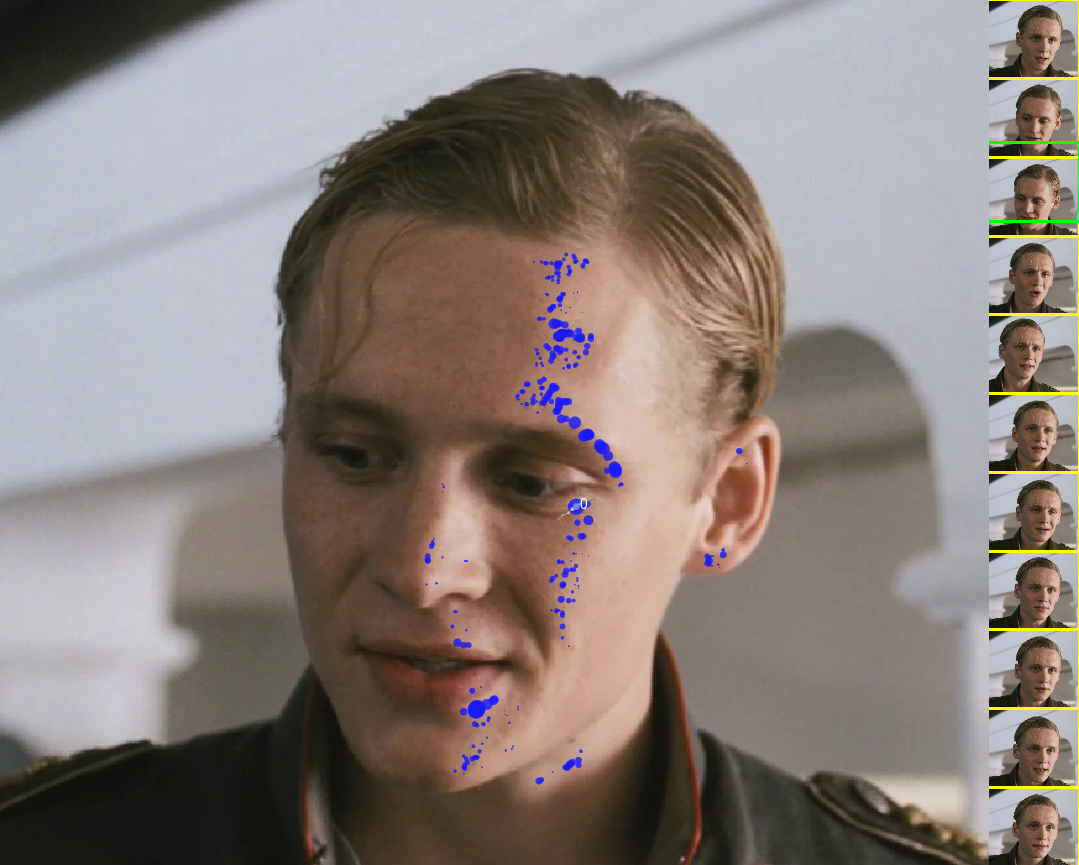
\includegraphics[width=0.40\linewidth]{candidates_lips_ridge_left_no_bg} \\[2em]
%\begin{sideways}{\makebox[0.32\linewidth][c]{Flank of a giraffe}}\end{sideways} & 
%\includegraphics[width=0.40\linewidth]{candidates_giraffes_flank_bg}&
%\includegraphics[width=0.40\linewidth]{candidates_giraffes_flank_no_bg}\\
\end{tabular}
   \vspace{0.3em}
  }\label{Future Work}

%%%%%%%%%%%%%%%%%%%%%%%%%%%%%%%%%%%%%%%%%%%%%%%%%%%%%%%%%%%%%%%%%%%%%%%%%%%%%%
  \headerbox{References}{name=applications,column=3,above=bottom,below=future work}{
%%%%%%%%%%%%%%%%%%%%%%%%%%%%%%%%%%%%%%%%%%%%%%%%%%%%%%%%%%%%%%%%%%%%%%%%%%%%%%
  The source code and compiled executables with an interactive interface are available at \\
  \url{http://www.cs.unibas.ch/personen/amberg_brian/graphtrack}
   \vspace{0.3em}
  }\label{References}

\end{poster}

\end{document}
